\section{Students $\mathbf{t}$-distribution}
\noindent\rule[\linienAbstand]{\linewidth}{\linienDickeDick}

\begin{figure}[H]
  \centering
  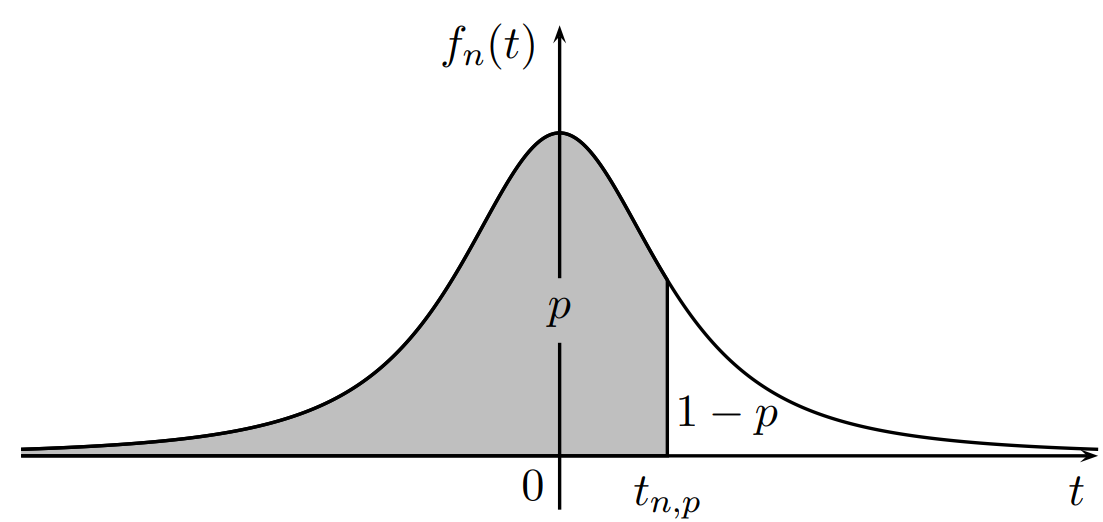
\includegraphics[width=.7\linewidth]{Pics/T.3.img.png}
\end{figure}
$p$-quantile $t_{n,p}$ for Student’s $t$-distribution with $n$ degrees of freedom. The density function is symmetric, therefore $t_{n,1-p} = -t_{n,p}$.
\begin{figure}[H]
  \centering
  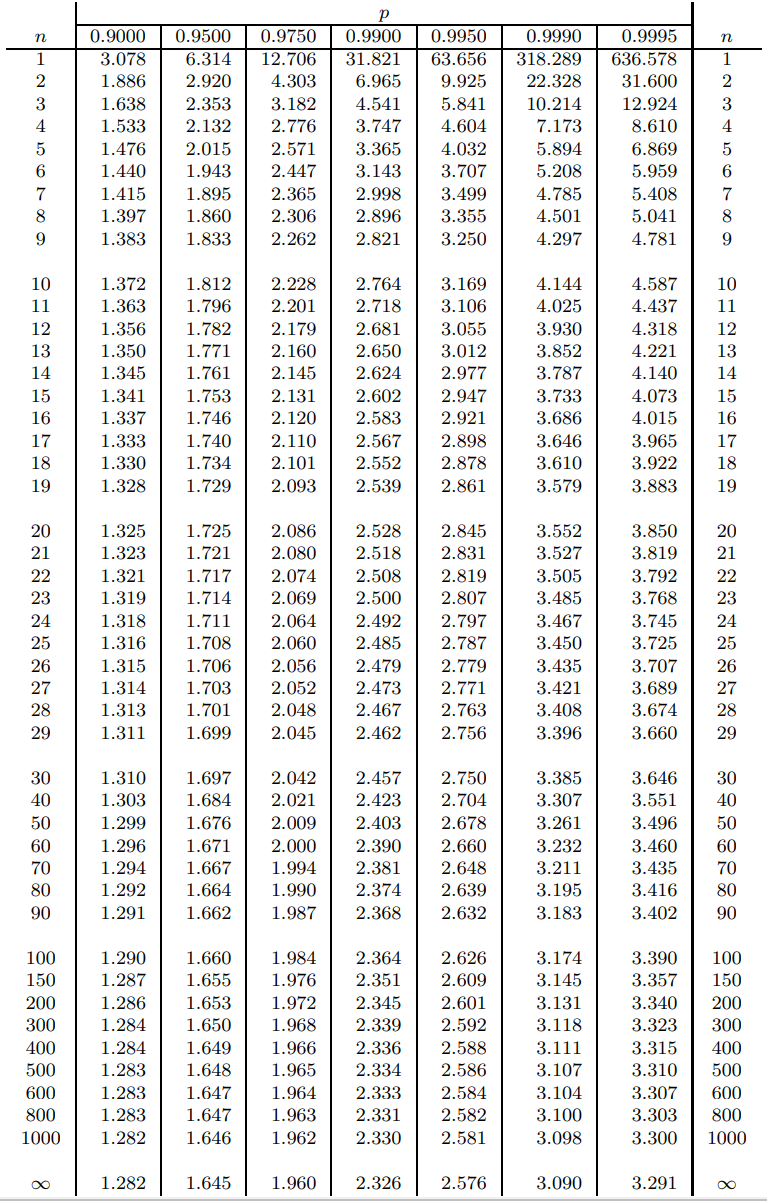
\includegraphics[width=\linewidth]{Pics/T.3.png}
\end{figure}

\section{Factors for constructing control charts}
\noindent\rule[\linienAbstand]{\linewidth}{\linienDickeDick}
\begin{figure}[H]
  \centering
  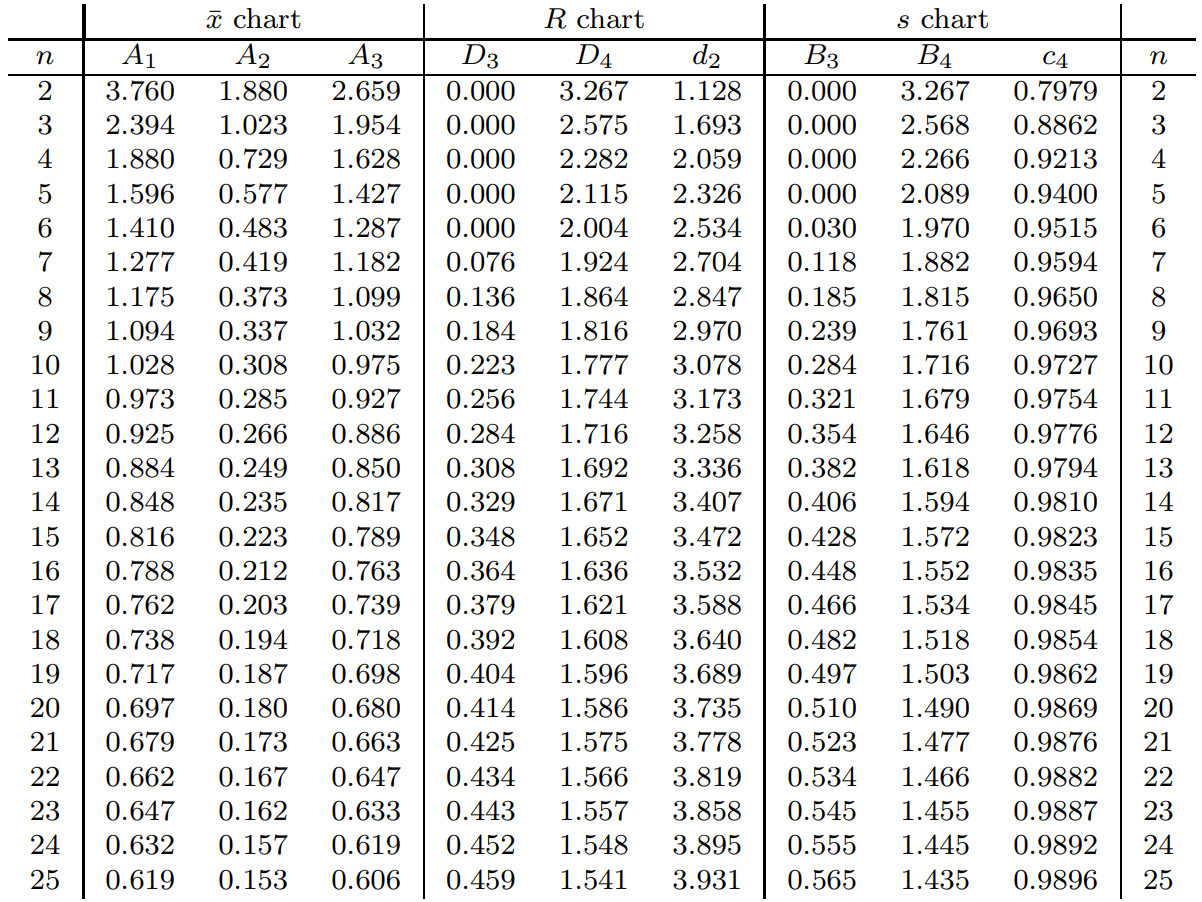
\includegraphics[width=\linewidth]{Pics/T.15.png}
\end{figure}
